\chapter{Analyse et spécification des besoins}

\section{Introduction}

Après avoir présenté, au chapitre précédent, le contexte général du projet ainsi que la solution retenue, ce chapitre a pour objectif de spécifier précisément les besoins auxquels la plateforme doit répondre, puis de fournir une vue d'ensemble de l'analyse globale du système et de son pilotage. Nous identifions dans un premier temps les différents acteurs qui interagissent avec le système, puis nous détaillons les besoins fonctionnels et non fonctionnels, ainsi que le diagramme de cas d'utilisation général. Nous présentons ensuite l'analyse globale de la plateforme (diagramme de classes d'analyse et architecture logique/physique), le pilotage du projet avec la méthode Scrum, avant de clore le chapitre par la description de l'environnement de travail utilisé pour la réalisation du projet.

\section{Modélisation du contexte}

\subsection{Identification des acteurs}

L'analyse de la documentation fonctionnelle de la plateforme permet d'identifier trois acteurs principaux, correspondant aux rôles gérés par le module de sécurité (Keycloak et couche d'autorisation applicative) :

\begin{itemize}[label=--]
\item Administrateur de la plateforme (ADMIN) : représente l'équipe opérationnelle de NextStep IT en charge de l'exploitation de la plateforme. Il supervise l'ensemble des clients (tenants), le cluster Kubernetes, la facturation globale, les quotas, et intervient via la console d'administration dédiée.

\item Administrateur de compte client (CLIENT\_ADMIN) : représente le responsable, côté client, d'un compte locataire de la plateforme. Il gère son équipe (invitation de membres), configure et déploie ses applications, consulte sa facturation, et dispose de la totalité des permissions sur les ressources de son compte.

\item Membre d'équipe (MEMBER) : utilisateur rattaché à un compte client, disposant d'un sous-ensemble de permissions accordées explicitement par le CLIENT\_ADMIN (par exemple : déployer une application, consulter les journaux, consulter la supervision, gérer Kafka ou l'Eventing), sans nécessairement disposer de l'ensemble des droits du compte.
\end{itemize}

\subsection{Spécification des besoins}
\label{sec:besoins-fonctionnels}

\medskip
\textbf{Besoins fonctionnels}
\medskip

Les besoins fonctionnels sont organisés ci-dessous selon les grands blocs fonctionnels et techniques de la plateforme, qui seront repris sous forme d'epics dans le Product Backlog présenté en section~\ref{sec:scrum}.

\begin{itemize}
    \item \textbf{Gestion des utilisateurs \& de l'authentification}
    \begin{itemize}[label=--]
        \item Inscription/connexion via Keycloak (SSO, OIDC).
        \item Modification du profil (email, mot de passe) synchronisée avec Keycloak.
    \end{itemize}

    \item \textbf{Gestion des déploiements d'applications}
    \begin{itemize}[label=--]
        \item Déployer une image Docker (Docker Hub ou registre privé) comme service serverless (Knative).
        \item Configuration : nom, image et tag, port, ressources CPU/RAM, réplicas minimum/maximum (scale-to-zero inclus).
        \item Suivi du statut en temps réel (RUNNING / SCALED\_TO\_ZERO / DEPLOYING / FAILED / SUSPENDED).
        \item Mise à jour d'une application (image, réplicas, ressources) et redéploiement.
        \item Retour (rollback) vers une révision antérieure.
        \item Suppression d'une application (libère les ressources Knative).
    \end{itemize}

    \item \textbf{Gestion de la messagerie Kafka \& de l'Eventing}
    \begin{itemize}[label=--]
        \item Création et gestion de sujets (topics) Kafka par tenant.
        \item Création de sources d'événements (KafkaSource) reliant un sujet à une application Knative.
        \item Création de déclencheurs (triggers Broker~$\rightarrow$~Subscriber) pour le routage d'événements CloudEvents.
    \end{itemize}

    \item \textbf{Gestion du monitoring \& des journaux}
    \begin{itemize}[label=--]
        \item Journaux de déploiement en temps réel (streaming SSE).
        \item Tableau de bord de métriques (CPU, RAM, requêtes/s) via Prometheus/Grafana.
        \item Alertes (échec de déploiement, boucle de redémarrage, dépassement de budget).
        \item Notifications in-app configurables par type d'événement.
    \end{itemize}

    \item \textbf{Gestion de la facturation \& du paiement}
    \begin{itemize}[label=--]
        \item Calcul du coût à l'usage (CPU-heure, RAM-heure) par application et par tenant.
        \item Génération automatique de factures mensuelles (1\textsuperscript{er} du mois).
        \item Paiement par carte bancaire (Stripe~\cite{StripeDoc}) — enregistrement de cartes, paiement de facture.
        \item Historique des transactions.
        \item Alerte J-3 avant échéance, passage automatique au statut OVERDUE en cas d'impayé.
        \item Suspension automatique du service en cas de facture impayée après échéance.
        \item Export du relevé de facturation (Excel).
    \end{itemize}

    \item \textbf{Gestion administrative (rôle ADMIN)}
    \begin{itemize}[label=--]
        \item Vue d'ensemble du cluster (nœuds, pods, namespaces, alertes actives).
        \item Gestion des clients : liste, suspension/restauration globale d'un compte.
        \item Gestion des quotas par tenant (CPU/RAM/nombre d'applications maximum) avec synchronisation des ResourceQuota Kubernetes.
        \item Gestion des applications tous tenants confondus (suppression forcée, suspension/restauration).
        \item Tableau de bord des revenus (facturation du mois en cours, projection de fin de mois, revenu par client, revenu Kafka).
        \item Génération manuelle des factures mensuelles (hors tâche planifiée).
        \item Suspension d'un service précis pour facture impayée.
        \item Journal d'audit des actions administratives (qui a fait quoi, quand), exportable en CSV.
    \end{itemize}
\end{itemize}

\medskip
\textbf{Besoins non fonctionnels}
\medskip

\begin{itemize}
    \item \textbf{Isolation multi-tenant}
    \begin{itemize}[label=--]
        \item Les ressources et les données d'un client ne doivent en aucun cas être accessibles par un autre client, ni par un tenant vers les composants internes de la plateforme (base de données, service d'authentification).
        \item Isolation au niveau applicatif : contrôle d'accès basé sur le propriétaire effectif de la ressource.
        \item Isolation au niveau réseau : règles d'isolation entre espaces de noms Kubernetes, appliquées automatiquement à la création de chaque namespace tenant.
        \item Isolation au niveau des droits d'accès au cluster : contrôle d'accès basé sur les rôles limitant le compte de service du backend aux seules ressources strictement nécessaires, secrets Kubernetes pour les identifiants sensibles.
    \end{itemize}

    \item \textbf{Élasticité et efficience des ressources}
    \begin{itemize}[label=--]
        \item Une application ne doit consommer aucune ressource de calcul lorsqu'elle est inactive (mise à l'échelle à zéro).
        \item La plateforme doit monter en charge automatiquement en fonction du trafic reçu, dans les bornes de réplicas configurées par le client.
        \item Le temps de réveil d'une application mise à l'échelle à zéro (cold start) doit rester acceptable pour l'utilisateur final.
    \end{itemize}

    \item \textbf{Sécurité}
    \begin{itemize}[label=--]
        \item L'authentification des utilisateurs doit reposer sur un fournisseur d'identité centralisé (Keycloak).
        \item Les autorisations doivent être vérifiées à chaque accès à une ressource, en fonction du rôle et du propriétaire effectif.
        \item Les échanges sensibles (jetons d'authentification, identifiants) ne doivent pas être exposés inutilement (journaux, paramètres d'URL, code source).
    \end{itemize}

    \item \textbf{Disponibilité}
    \begin{itemize}[label=--]
        \item Les composants de la plateforme elle-même (backend, portails, briques d'infrastructure) doivent pouvoir être redéployés sans interruption prolongée de service.
        \item Le système doit permettre de détecter automatiquement une dégradation (redémarrages en boucle, alertes) et, si possible, la corriger sans intervention manuelle.
    \end{itemize}

    \item \textbf{Observabilité}
    \begin{itemize}[label=--]
        \item L'état du système, à tous les niveaux (infrastructure, plateforme, applications clientes), doit pouvoir être supervisé au travers d'outils de métriques et de tableaux de bord (Prometheus/Grafana).
        \item Les journaux applicatifs et de déploiement doivent être consultables en temps réel.
        \item Les actions administratives sensibles doivent être tracées dans un journal d'audit consultable a posteriori.
    \end{itemize}

    \item \textbf{Automatisation}
    \begin{itemize}[label=--]
        \item La construction, la publication et le déploiement des composants de la plateforme doivent être automatisés à chaque évolution du code source.
        \item L'automatisation doit couvrir l'ensemble des composants déployables de la plateforme (backend, portail client, console d'administration).
    \end{itemize}
\end{itemize}

\subsection{Diagramme de cas d'utilisation général}
Dans cette section, nous décrivons les exigences du système de manière formelle à l'aide des deux diagrammes de cas d'utilisation ci-dessous (figures~\ref{fig:uc-global} et~\ref{fig:uc-global-admin}), qui couvrent respectivement les rôles CLIENT\_ADMIN/MEMBER et le rôle ADMIN.

\begin{figure}[H]
 \centering
    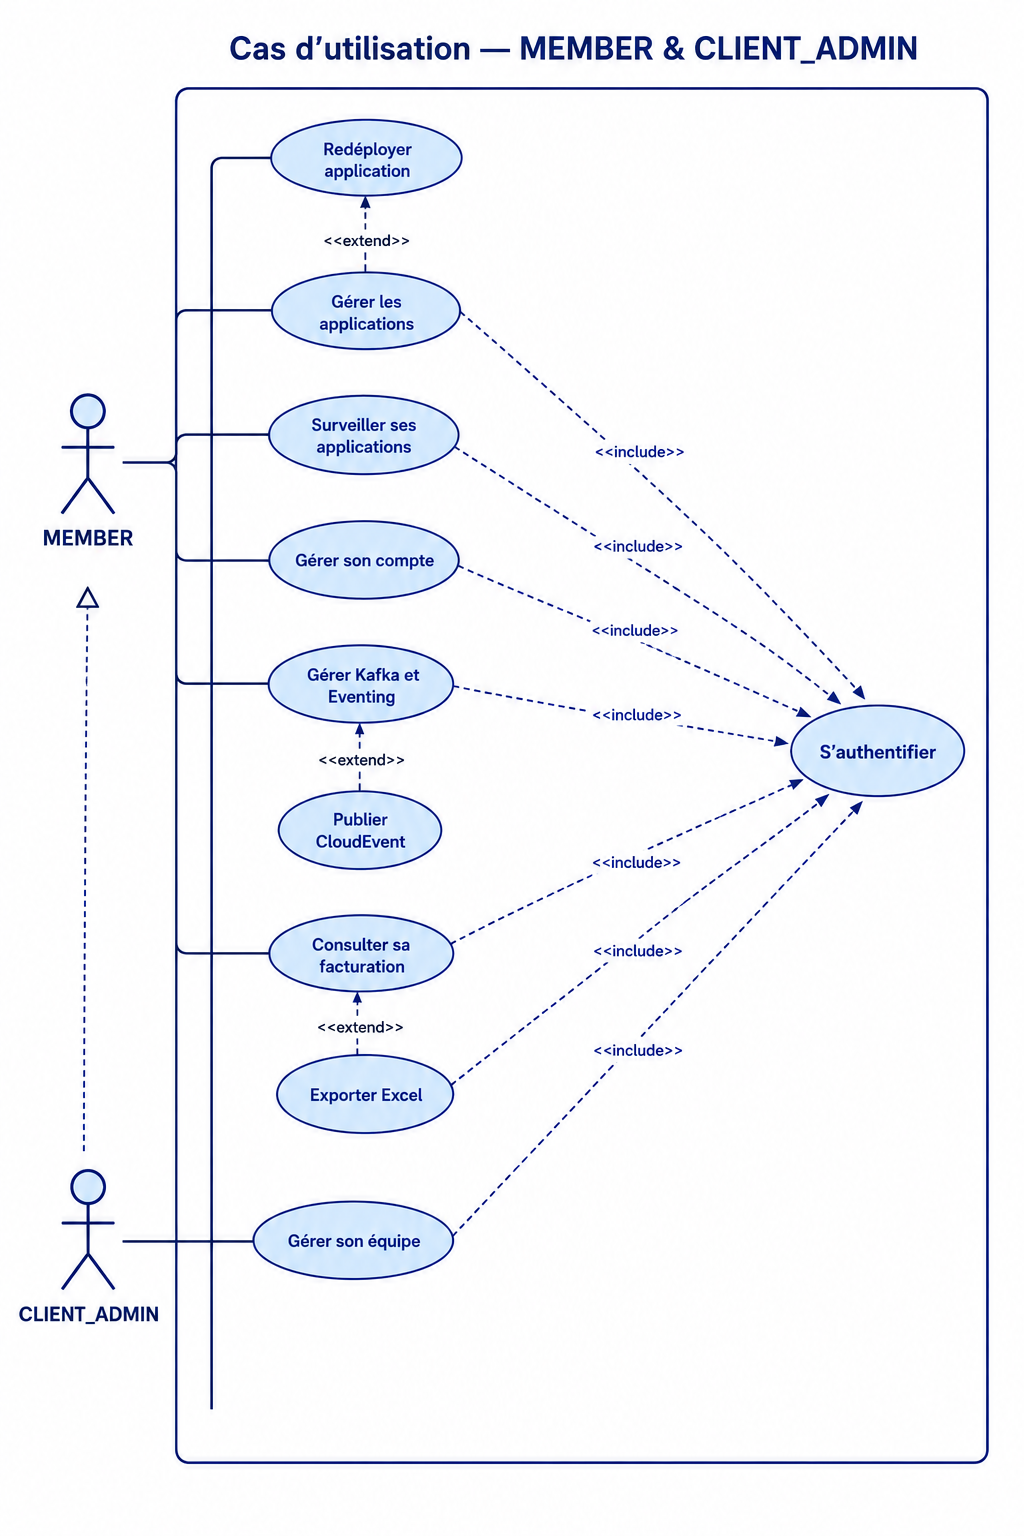
\includegraphics[width=13cm]{image/usescasememeberadmin.png}
    \caption{Diagramme de cas d'utilisation global de la plateforme — CLIENT\_ADMIN et MEMBER}
    \label{fig:uc-global}
\end{figure}

\begin{figure}[H]
 \centering
    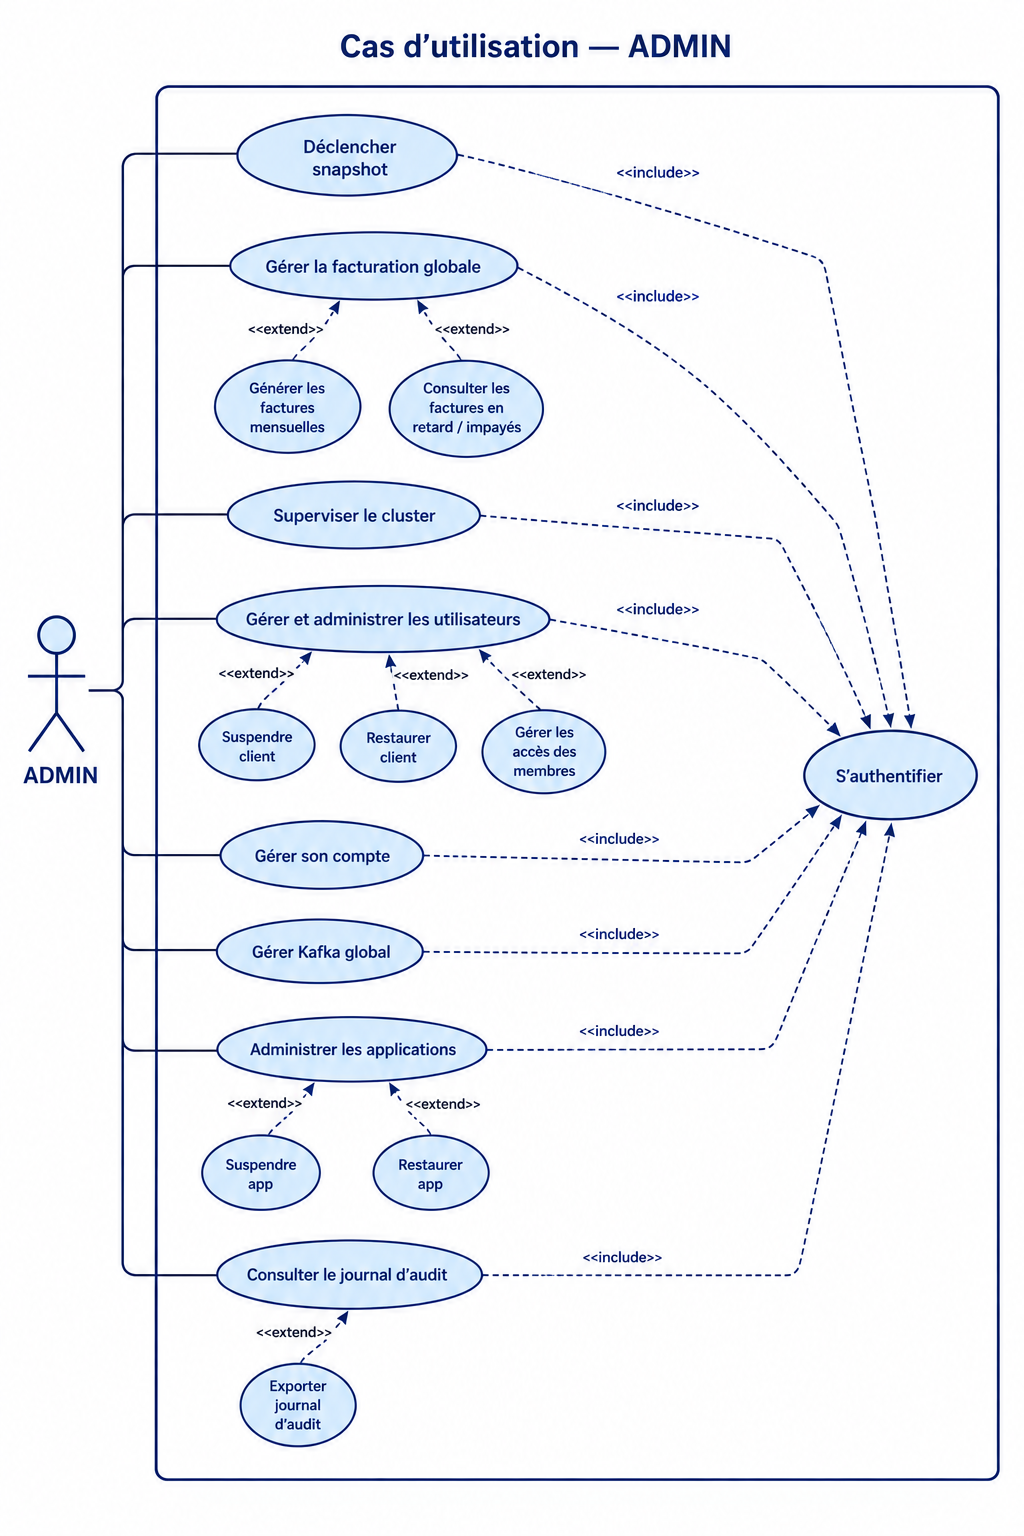
\includegraphics[width=13cm]{image/diagrameadmin.png}
    \caption{Diagramme de cas d'utilisation global de la plateforme — ADMIN}
    \label{fig:uc-global-admin}
\end{figure}

\section{Analyse Globale}

Cette section donne une vue d'ensemble cohérente de l'architecture logique et physique du système, des composants qui le constituent et de leurs interactions, ainsi que des processus métier les plus structurants, indépendamment du découpage en sprints qui structurera les chapitres suivants. Les diagrammes UML propres à une fonctionnalité particulière (par exemple le diagramme de séquence détaillé de la création d'un déclencheur Kafka) seront présentés dans le chapitre de réalisation correspondant, en cohérence avec la vue d'ensemble donnée ici.

\subsection{Diagramme de classes d'analyse}

La figure~\ref{fig:classes-global} présente les principales entités métier du système et leurs relations : \texttt{User}, \texttt{App}, \texttt{DeploymentLog}, \texttt{BillingSnapshot}, \texttt{AppInvoice} et les clés d'API. La propriété des applications est gérée par \texttt{UserContextService}, qui rattache les ressources d'un \texttt{MEMBER} à son \texttt{CLIENT\_ADMIN}.

\begin{figure}[H]
 \centering
    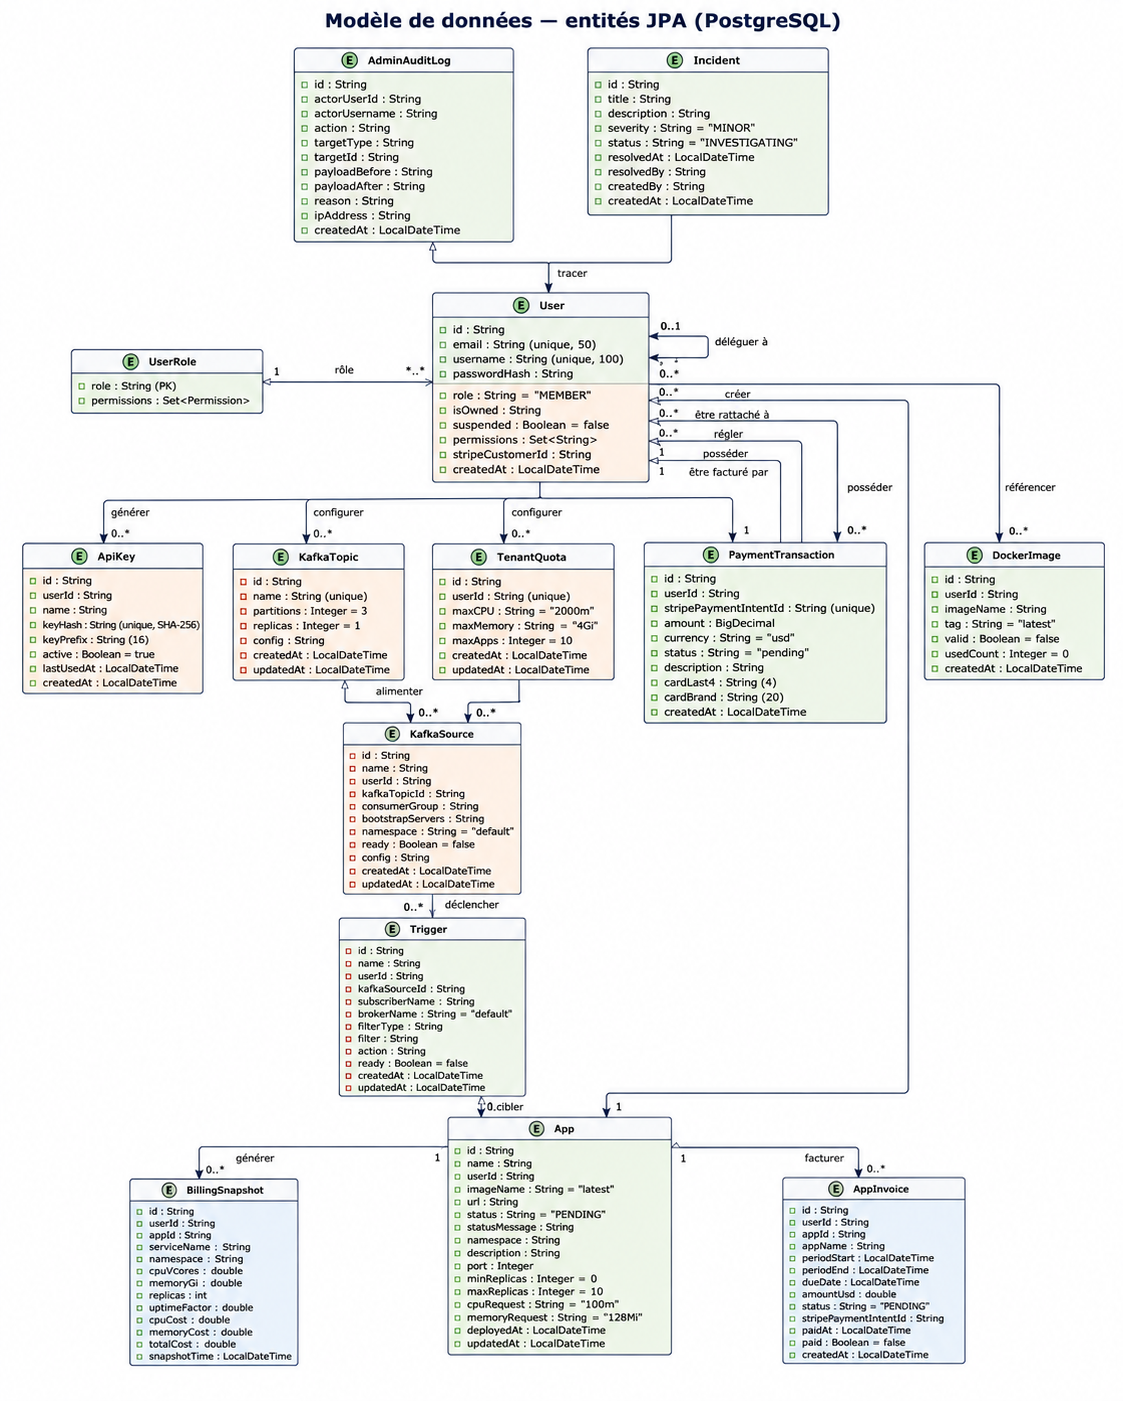
\includegraphics[width=13.5cm]{image/class1.png}
    \caption{Diagramme de classe d'analyse global}
    \label{fig:classes-global}
\end{figure}

\subsection{Architecture globale}

\subsubsection{Architecture logique de la plateforme}

L'architecture logique de la plateforme est organisée en trois couches, représentées à la figure ~\ref{fig:architecture-logique} :

\begin{figure}[H]
\centering
    
\includegraphics[width=13.5cm]{image/architecture_logique.png}
    \caption{Architecture logique de la plateforme}
    \label{fig:architecture-logique}
\end{figure}


\begin{itemize}
    \item \textbf{Présentation} : deux applications React distinctes, servies via Nginx. Le portail client couvre le déploiement et le suivi des applications, la facturation et la gestion d'équipe ; la console d'administration donne à l'équipe NextStep IT une vue sur l'ensemble des clients et du cluster.
    \item \textbf{Service} : une seule API REST en Spring Boot, découpée par domaine métier (applications, sécurité, Kafka, facturation, administration...). C'est elle qui concentre toute la logique et qui parle au cluster, via Fabric8 — une bibliothèque Java exécutée dans son propre processus, pas un service séparé.
    \item \textbf{Infrastructure} : le cluster Kubernetes et ses opérateurs (Knative pour l'exécution serverless, Strimzi pour Kafka), la couche réseau (Cilium en CNI, Kourier en passerelle d'entrée), et les briques transverses Keycloak, PostgreSQL, Prometheus/Grafana.
\end{itemize}

Seul le backend parle à l'API Kubernetes : ni les portails ni un système externe (un pipeline CI/CD, par exemple) n'y accèdent directement. Toute action passe donc par cette couche de service, qui applique l'authentification et l'isolation entre tenants avant d'agir sur le cluster.

\subsubsection{Architecture physique de la plateforme}

Au-delà de son organisation logique, il est utile de voir comment la plateforme se répartit concrètement sur le cluster une fois en fonctionnement. La figure~\ref{fig:archi-physique} reprend, namespace par namespace, ce qui a pu être observé directement sur le cluster décrit en section~\ref{sec:env-materiel} — les pods réellement en cours d'exécution, et non une simple projection théorique du déploiement.

\begin{figure}[H]
\centering
    
\includegraphics[width=13.5cm]{image/architecture_physique.png}
    \caption{Architecture physique de l'infrastructure Kubernetes}
    \label{fig:archi-physique}
\end{figure}

Le cluster s'appuie sur trois nœuds Ubuntu. \texttt{vm01} porte le plan de contrôle Kubernetes (\texttt{kube-apiserver}, \texttt{etcd}, \texttt{kube-scheduler}, \texttt{kube-controller-manager}), tandis que \texttt{vm02} et \texttt{vm03} font tourner l'ensemble des pods, ceux de la plateforme comme ceux des applications clientes.

En façade, trois composants réseau se partagent des rôles bien distincts. MetalLB attribue une adresse IP de type \texttt{LoadBalancer} à chaque \texttt{Service} Kubernetes qui en a besoin ; Kourier se contente de router le trafic HTTP vers les applications Knative des tenants ; Cilium, lui, assure la connectivité des pods en tant que CNI du cluster et applique les \texttt{NetworkPolicy}. Le backend et les portails, exposés directement en \texttt{Service} \texttt{LoadBalancer}, reçoivent donc leur IP de MetalLB sans jamais transiter par Kourier.

Le namespace \texttt{platform} regroupe les deux composants centraux de la plateforme : PostgreSQL, avec son volume persistant, et le backend Spring Boot. Ce dernier tourne en \texttt{Deployment} Kubernetes classique plutôt qu'en service Knative, car il doit rester disponible en permanence et ne se prête pas à une mise à l'échelle à zéro.

Vient ensuite le middleware Cloud Native. Le broker Kafka, opéré par Strimzi, est une instance unique du cluster, mutualisée entre tous les tenants. Il en va de même pour le plan de contrôle de Knative Eventing (le contrôleur Eventing et le dispatcher de sources Kafka), qui tourne une seule fois pour tout le cluster plutôt que d'être dupliqué par client — à la différence des ressources Broker et Trigger elles-mêmes, qui sont instanciées séparément dans le namespace de chaque tenant. Cette mutualisation du plan de contrôle a une conséquence concrète : lorsque le dispatcher de sources Kafka a connu un incident, la livraison d'événements s'est interrompue pour tous les clients à la fois, pas seulement pour l'un d'eux.

Enfin, chaque client dispose de son propre namespace \texttt{user-<client>}, créé automatiquement lors de son premier déploiement et isolé par une \texttt{NetworkPolicy} générée à la volée. C'est là que vivent ses applications, sous forme de ressources Knative Service donnant naissance à des Revisions puis à des pods applicatifs.

\section{Pilotage du projet avec SCRUM}
\label{sec:scrum}

Le cadre agile Scrum, retenu au chapitre précédent pour la conduite de ce projet, structure le développement en itérations courtes et fixes appelées sprints, à l'issue desquelles un incrément de produit potentiellement livrable est produit.

Dans les tableaux de backlog présentés dans ce chapitre et les suivants, chaque tâche est associée à une estimation exprimée sur une échelle de complexité relative à trois niveaux : \textbf{1} (faible complexité — modification simple ou localisée), \textbf{2} (complexité moyenne — développement impliquant plusieurs composants ou une logique métier non triviale) et \textbf{3} (complexité élevée — intégration de plusieurs systèmes, gestion d'états asynchrones ou risques techniques significatifs).

\subsection{Backlog du produit}

Le tableau~\ref{tab:backlog} présente le backlog du produit de la plateforme. Les fonctionnalités sont organisées par module (en cohérence directe avec les besoins fonctionnels spécifiés en section~\ref{sec:besoins-fonctionnels}) et décrites sous forme de User Stories.

{
\setlength{\tabcolsep}{4pt}
\renewcommand{\arraystretch}{1.5}
\begin{longtable}{|>{\centering\arraybackslash}m{1.1cm}|>{\centering\arraybackslash}m{2.9cm}|>{\centering\arraybackslash}m{1.4cm}|>{\raggedright\arraybackslash}p{6.6cm}|>{\centering\arraybackslash}m{2.3cm}|}
\hline
ID & Module & ID US & User Story & Complexité\\
\hline
\endfirsthead

\hline
ID & Module & ID US & User Story & Complexité\\
\hline
\endhead

\hline
\multicolumn{5}{r}{Suite à la page suivante}\\
\endfoot

\endlastfoot

\multirow{4}{*}{M1} & \multirow{4}{2.9cm}{\centering Authentification \& Sécurité} & M1.1 & En tant qu'ADMIN, CLIENT\_ADMIN ou MEMBER, je souhaite me connecter à la plateforme via Keycloak. & Moyenne\\
\cline{3-5}
&& M1.2 & En tant qu'ADMIN, CLIENT\_ADMIN ou MEMBER, je souhaite me déconnecter du système. & Faible\\
\cline{3-5}
&& M1.3 & En tant qu'ADMIN, CLIENT\_ADMIN ou MEMBER, je souhaite que mon jeton d'authentification (JWT) soit automatiquement rafraîchi. & Moyenne\\
\cline{3-5}
&& M1.4 & En tant qu'ADMIN, je souhaite définir les rôles et les permissions des utilisateurs. & Élevée\\
\hline

\multirow{4}{*}{M2} & \multirow{4}{2.9cm}{\centering Utilisateurs \& équipes} & M2.1 & En tant que CLIENT\_ADMIN, je souhaite inviter un membre dans mon équipe. & Moyenne\\
\cline{3-5}
&& M2.2 & En tant que CLIENT\_ADMIN, je souhaite modifier les permissions d'un membre de mon équipe. & Moyenne\\
\cline{3-5}
&& M2.3 & En tant que CLIENT\_ADMIN, je souhaite retirer un membre de mon équipe. & Faible\\
\cline{3-5}
&& M2.4 & En tant qu'ADMIN, je souhaite gérer les comptes clients (activation, suspension, quotas). & Élevée\\
\hline

\multirow{3}{*}{M3} & \multirow{3}{2.9cm}{\centering Infrastructure Cloud Native} & M3.1 & En tant que système, je souhaite créer automatiquement un espace de noms (namespace) dédié pour chaque nouveau tenant. & Élevée\\
\cline{3-5}
&& M3.2 & En tant que système, je souhaite appliquer automatiquement une NetworkPolicy isolant chaque tenant. & Élevée\\
\cline{3-5}
&& M3.3 & En tant qu'ADMIN, je souhaite superviser l'état des nœuds du cluster Kubernetes. & Moyenne\\
\hline

\multirow{1}{*}{M4} & \multirow{1}{2.9cm}{\centering Gestion des applications} & M4.1 & En tant que CLIENT\_ADMIN ou MEMBER, je souhaite déployer une application à partir d'une image Docker. & Élevée\\
\cline{3-5}
&& M4.2 & En tant que CLIENT\_ADMIN ou MEMBER, je souhaite définir les ressources (CPU, mémoire) et les bornes de mise à l'échelle de mon application. & Moyenne\\
\cline{3-5}
&& M4.3 & En tant que CLIENT\_ADMIN ou MEMBER, je souhaite mettre à jour la configuration d'une application déjà déployée. & Moyenne\\
\cline{3-5}
&& M4.4 & En tant que CLIENT\_ADMIN ou MEMBER, je souhaite supprimer une application (suppression logique, conservation de l'historique de facturation). & Moyenne\\
\cline{3-5}
&& M4.5 & En tant que CLIENT\_ADMIN ou MEMBER, je souhaite consulter l'historique des révisions d'une application. & Moyenne\\
\cline{3-5}
&& M4.6 & En tant que CLIENT\_ADMIN ou MEMBER, je souhaite effectuer un rollback vers une révision antérieure. & Élevée\\
\cline{3-5}
&& M4.7 & En tant que CLIENT\_ADMIN ou MEMBER, je souhaite suivre en temps réel le statut de déploiement de mon application. & Élevée\\
\hline

\multirow{3}{*}{M5} & \multirow{3}{2.9cm}{\centering Messaging Kafka} & M5.1 & En tant que CLIENT\_ADMIN ou MEMBER, je souhaite créer un sujet (topic) Kafka pour mon compte. & Moyenne\\
\cline{3-5}
&& M5.2 & En tant que CLIENT\_ADMIN ou MEMBER, je souhaite consulter la liste des sujets Kafka de mon compte. & Faible\\
\cline{3-5}
&& M5.3 & En tant que CLIENT\_ADMIN ou MEMBER, je souhaite supprimer un sujet Kafka. & Faible\\
\hline

\multirow{3}{*}{M6} & \multirow{3}{2.9cm}{\centering Knative Eventing} & M6.1 & En tant que CLIENT\_ADMIN ou MEMBER, je souhaite relier un sujet Kafka à une de mes applications déployées. & Élevée\\
\cline{3-5}
&& M6.2 & En tant que CLIENT\_ADMIN ou MEMBER, je souhaite que mon application soit automatiquement réveillée (scale depuis zéro) à la réception d'un événement. & Élevée\\
\cline{3-5}
&& M6.3 & En tant que CLIENT\_ADMIN ou MEMBER, je souhaite configurer un déclencheur (Trigger) avec un filtre sur le type d'événement. & Moyenne\\
\hline

\multirow{3}{*}{M7} & \multirow{3}{2.9cm}{\centering Facturation} & M7.1 & En tant que CLIENT\_ADMIN ou MEMBER, je souhaite consulter la facturation de mes applications basée sur leur usage réel. & Élevée\\
\cline{3-5}
&& M7.2 & En tant qu'ADMIN, je souhaite consulter la facturation globale de tous les comptes clients. & Moyenne\\
\cline{3-5}
&& M7.3 & En tant que CLIENT\_ADMIN ou MEMBER, je souhaite recevoir une alerte lorsque mon budget approche un seuil défini. & Moyenne\\
\hline

\multirow{4}{*}{M8} & \multirow{4}{2.9cm}{\centering Monitoring \& Observabilité} & M8.1 & En tant que CLIENT\_ADMIN ou MEMBER, je souhaite consulter les journaux applicatifs de mon application en temps réel (SSE). & Élevée\\
\cline{3-5}
&& M8.2 & En tant que CLIENT\_ADMIN ou MEMBER, je souhaite consulter les métriques (CPU, mémoire, requêtes) de mon application. & Moyenne\\
\cline{3-5}
&& M8.3 & En tant que CLIENT\_ADMIN ou MEMBER, je souhaite être alerté automatiquement en cas de redémarrage en boucle (crash loop) d'une application. & Élevée\\
\cline{3-5}
&& M8.4 & En tant qu'ADMIN, je souhaite consulter un tableau de bord Grafana de l'état global du cluster. & Moyenne\\
\hline

\multirow{2}{*}{M9} & \multirow{2}{2.9cm}{\centering Administration plateforme} & M9.1 & En tant qu'ADMIN, je souhaite consulter le journal d'audit des actions effectuées sur la plateforme. & Moyenne\\
\cline{3-5}
&& M9.2 & En tant qu'ADMIN, je souhaite gérer les quotas alloués à chaque compte client. & Moyenne\\
\hline

\multirow{3}{*}{M10} & \multirow{3}{2.9cm}{\centering CI/CD} & M10.1 & En tant qu'équipe de développement de la plateforme, je souhaite que chaque évolution du code source déclenche automatiquement la construction d'une image Docker via Kaniko. & Élevée\\
\cline{3-5}
&& M10.2 & En tant qu'équipe de développement de la plateforme, je souhaite que l'image construite soit automatiquement publiée sur le registre Docker Hub. & Moyenne\\
\cline{3-5}
&& M10.3 & En tant qu'équipe de développement de la plateforme, je souhaite que la nouvelle version soit automatiquement déployée sur le cluster après publication. & Élevée\\
\hline
\caption{Backlog du produit}
\label{tab:backlog}
\end{longtable}
}

\subsection{Planification des Sprints}

La planification cible retenue pour la conduite du projet, définissant l'ordre logique de construction des différentes briques de la plateforme, est présentée dans le tableau~\ref{tab:sprints}. Cette planification a servi de cadre méthodologique tout au long du projet ; elle reflète la démarche adoptée plutôt qu'un journal exhaustif et daté de chaque tâche réalisée, celui-ci n'ayant pas fait l'objet d'une documentation formelle systématique sprint par sprint.

\begin{table}[H]
\centering
\renewcommand{\arraystretch}{1.3}
\begin{tabular}{|p{3cm}|p{10cm}|}
\hline
Sprint & Objectif principal \\
\hline
Sprint 0  & Infrastructure Kubernetes \\
\hline
Sprint 1  & Knative Serving \\
\hline
Sprint 2  & Kafka \& Strimzi \\
\hline
Sprint 3  & Gestion des utilisateurs et des accès (backend + portail) \\
\hline
Sprint 4  & Gestion des applications (backend + portail) et début du pipeline CI/CD Backend \\
\hline
Sprint 5  & Gestion de la messagerie événementielle : Kafka et Knative Eventing (backend + portail) \\
\hline
Sprint 6  & Gestion de l'observabilité applicative (backend + portail) \\
\hline
Sprint 7  & Gestion de la facturation et des paiements (backend + portail) \\
\hline
Sprint 8  & Gestion des comptes clients, des quotas et de l'audit \\
\hline
Sprint 9  & Gestion de l'exploitation du cluster et du statut public \\
\hline
Sprint 10 & Durcissement et sécurité \\
\hline
Sprint 11 & Pipeline CI/CD complet \\
\hline
\end{tabular}
\caption{Planification des sprints du projet}
\label{tab:sprints}
\end{table}

Le détail de la réalisation de chacun de ces sprints (analyse, conception et implémentation) est présenté progressivement dans les chapitres suivants, regroupés par release. Conformément aux besoins fonctionnels spécifiés en section~\ref{sec:besoins-fonctionnels} (portail client et console d'administration comme composants à part entière de la plateforme, au même titre que le backend), chaque sprint à partir du Sprint 3 livre conjointement la brique backend et l'interface graphique correspondante, plutôt que de reporter l'ensemble du développement frontend à la fin du projet.

\section{Environnement de travail}

\subsection{Environnement matériel de développement}
\label{sec:env-materiel}

\subsubsection{Poste de développement}

Le développement de la plateforme (backend, portails web, manifestes Kubernetes) a été réalisé sur un poste de travail disposant des caractéristiques suivantes :

\begin{itemize}
    \item Modèle : Ordinateur portable MSI GF63 Thin 10SC
    \item Système d'exploitation : Windows 11 Pro (64 bits)
    \item Processeur : Intel(R) Core(TM) i7-10750H CPU @ 2.60GHz
    \item Mémoire RAM : 16 Go
    \item Stockage : 2 $\times$ SSD 512 Go (TEAM T253 512GB + Micron 2210 512GB), soit environ 1 To au total
\end{itemize}

\subsubsection{Cluster de déploiement (infrastructure Kubernetes)}

Le déploiement et l'exploitation de la plateforme se sont appuyés sur un cluster Kubernetes composé de trois machines virtuelles sous Ubuntu 24, administrées via un utilisateur \texttt{sysadmin} : un nœud de plan de contrôle (control-plane) et deux nœuds de travail (workers), sur lesquels sont exécutés l'ensemble des composants de la plateforme ainsi que les applications des clients.

\begin{table}[H]
\centering
\renewcommand{\arraystretch}{1.3}
\begin{tabular}{|l|p{4cm}|c|p{5cm}|}
\hline
\textbf{Nom de la VM} & \textbf{Ressources} & \textbf{Système} & \textbf{Rôle} \\
\hline
Master   & 4 vCPU, 8 Go RAM, 50 Go disque & Ubuntu 24 & Plan de contrôle (control-plane) \\
\hline
Worker 1 & 4 vCPU, 8 Go RAM, 50 Go disque & Ubuntu 24 & Nœud de travail \\
\hline
Worker 2 & 4 vCPU, 8 Go RAM, 50 Go disque & Ubuntu 24 & Nœud de travail \\
\hline
\end{tabular}
\caption{Caractéristiques des machines virtuelles du cluster Kubernetes}
\label{tab:vms-cluster}
\end{table}

Le cluster utilise Cilium comme interface réseau de conteneurs (CNI), MetalLB pour l'attribution d'adresses IP aux services de type LoadBalancer dans un environnement dépourvu de répartiteur de charge natif, et Kourier comme passerelle d'entrée (ingress gateway) pour Knative Serving.

\subsection{Environnement logiciel de développement}

\subsubsection{Langages de programmation}

Le choix des langages de programmation est basé sur les exigences techniques de la plateforme : performance et sécurité du backend, réactivité des interfaces web, et portabilité des scripts d'exploitation du cluster. Le tableau~\ref{tab:langages} présente les langages utilisés.

\renewcommand{\arraystretch}{1.3}
\begin{center}
\begin{tabular}{|m{3cm}|m{10cm}|}
\hline
\centering Langage & \centering\arraybackslash Description \\
\hline
Java & Langage principal du backend applicatif (\texttt{backend-api}), développé avec Spring Boot. \\
\hline
TypeScript / JavaScript & Langages utilisés pour le développement des deux portails web React (\texttt{web-portal} et \texttt{admin-console}). \\
\hline
YAML & Langage de description déclarative utilisé pour l'ensemble des manifestes Kubernetes, Knative, Strimzi, ainsi que pour la configuration de l'application (\texttt{application.yml}). \\
\hline
Shell (Bash) & Utilisé pour les scripts de déploiement, d'initialisation du cluster et d'automatisation des tâches d'exploitation. \\
\hline
Groovy & Langage utilisé pour l'écriture des Jenkinsfiles du pipeline CI/CD. \\
\hline
\end{tabular}
\captionof{table}{Langages de programmation utilisés}
\label{tab:langages}
\end{center}

\vspace{1em}

\subsubsection{Frameworks et bibliothèques}

Les frameworks et bibliothèques retenus ont été sélectionnés pour leur maturité, leur performance et leur adéquation aux besoins fonctionnels de la plateforme. Le tableau~\ref{tab:frameworks} en présente une synthèse.

\renewcommand{\arraystretch}{1.3}
\begin{center}
\begingroup
\centering
\renewcommand{\arraystretch}{1.2}
\begin{longtable}{|m{3cm}|m{11.5cm}|}
\caption{Frameworks et bibliothèques utilisés}
\label{tab:frameworks}\\
\hline
\multicolumn{1}{|c|}{\textbf{Framework}} & \multicolumn{1}{c|}{\textbf{Description}} \\
\hline
\endfirsthead

\multicolumn{2}{l}{\small\itshape (suite du tableau~\ref{tab:frameworks})}\\
\hline
\multicolumn{1}{|c|}{\textbf{Framework}} & \multicolumn{1}{c|}{\textbf{Description}} \\
\hline
\endhead

\hline
\multicolumn{2}{r}{\small\itshape (suite page suivante)}\\
\endfoot

\hline
\endlastfoot

Spring Boot & Framework backend utilisé pour l'exposition de l'API REST, l'injection de dépendances, la sécurité (Spring Security) et l'accès aux données (Spring Data JPA). \\
\hline
Fabric8 Kubernetes Client & Bibliothèque Java utilisée par le backend pour orchestrer les ressources Kubernetes natives et les ressources personnalisées (CRD) de Knative Serving, Knative Eventing et Strimzi. \\
\hline
Kafka Clients (Apache Kafka) & Bibliothèque cliente utilisée par le backend (API Admin Kafka) pour créer et gérer les sujets (topics) des tenants. \\
\hline
React & Bibliothèque utilisée pour le développement des interfaces graphiques du portail client et de la console d'administration. \\
\hline
PostgreSQL / JPA-Hibernate & Système de gestion de base de données relationnelle et couche de mapping objet-relationnel utilisés pour la persistance des entités métier. \\
\hline
Keycloak (OpenID Connect) & Bibliothèque d'intégration utilisée côté backend et frontend pour l'authentification et la validation des jetons JWT. \\
\hline
\end{longtable}
\endgroup
\end{center}

\vspace{1em}

\subsubsection{Outils de développement et de modélisation}

Le tableau~\ref{tab:outils-dev} présente les outils utilisés pour l'écriture du code, la gestion de versions, les tests manuels d'API et la modélisation UML du présent mémoire.

\begingroup
\centering
\renewcommand{\arraystretch}{1.2}
\begin{longtable}{|m{3cm}|m{11.5cm}|}
\caption{Outils de développement et de modélisation utilisés}
\label{tab:outils-dev}\\
\hline
\multicolumn{1}{|c|}{\textbf{Outil}} & \multicolumn{1}{c|}{\textbf{Description}} \\
\hline
\endfirsthead

\multicolumn{2}{l}{\small\itshape (suite du tableau~\ref{tab:outils-dev})}\\
\hline
\multicolumn{1}{|c|}{\textbf{Outil}} & \multicolumn{1}{c|}{\textbf{Description}} \\
\hline
\endhead

\hline
\multicolumn{2}{r}{\small\itshape (suite page suivante)}\\
\endfoot

\hline
\endlastfoot

Visual Studio Code & Environnement de développement intégré léger et extensible, utilisé pour le développement du backend Spring Boot, des deux applications frontend React, ainsi que pour la rédaction des manifestes Kubernetes et des scripts de déploiement. \\
\hline
GitHub & Plateforme d'hébergement du code source et de gestion de versions, utilisée pour le suivi des évolutions du projet et le déclenchement des pipelines d'intégration continue. \\
\hline
Postman & Outil de test et de documentation des API REST, utilisé pour valider manuellement le comportement des différents points d'accès exposés par le backend avant leur intégration dans les interfaces graphiques. \\
\hline
PlantUML~\cite{PlantUMLDoc} & Outil de modélisation UML en tant que code, utilisé pour la production des diagrammes de cas d'utilisation, de classes, de composants, de déploiement et de séquence présentés dans ce mémoire, à partir de scripts textuels versionnés avec le code source. \\
\hline
\end{longtable}
\endgroup

\vspace{1em}

\subsubsection{Outils DevOps et déploiement}

La mise en production de la plateforme repose sur une chaîne DevOps automatisée garantissant la fiabilité et la répétabilité des déploiements. Le tableau~\ref{tab:outils-devops} présente les outils utilisés pour la conteneurisation, l'intégration continue et l'exploitation du cluster.

\renewcommand{\arraystretch}{1.3}

\begingroup
\centering
\renewcommand{\arraystretch}{1.2}
\begin{longtable}{|m{3cm}|m{11.5cm}|}
\caption{Outils DevOps et de déploiement utilisés}
\label{tab:outils-devops}\\
\hline
\multicolumn{1}{|c|}{\textbf{Outil}} & \multicolumn{1}{c|}{\textbf{Description}} \\
\hline
\endfirsthead

\multicolumn{2}{l}{\small\itshape (suite du tableau~\ref{tab:outils-devops})}\\
\hline
\multicolumn{1}{|c|}{\textbf{Outil}} & \multicolumn{1}{c|}{\textbf{Description}} \\
\hline
\endhead

\hline
\multicolumn{2}{r}{\small\itshape (suite page suivante)}\\
\endfoot

\hline
\endlastfoot

Docker & Utilisé pour la construction et l'exécution locale des images de conteneurs avant leur publication sur le registre Docker Hub par la chaîne CI/CD. \\
\hline
Jenkins et Kaniko & Utilisés pour l'automatisation de la construction, de la publication et du déploiement continu des composants de la plateforme, Kaniko permettant de construire les images sans démon Docker privilégié à l'intérieur du cluster. \\
\hline
kubectl & Interface en ligne de commande de Kubernetes, utilisée quotidiennement pour l'inspection de l'état du cluster, le déploiement manuel de ressources lors des phases de mise au point, et le diagnostic des incidents. \\
\hline
\end{longtable}
\endgroup
\section{Conclusion}

Ce chapitre a permis de formaliser les besoins fonctionnels et non fonctionnels de la plateforme, de préciser les acteurs qui interagissent avec le système et le diagramme de cas d'utilisation général qui en découle, puis de présenter l'analyse globale de la plateforme (diagramme de classes, architecture logique et physique, processus métier principaux) et le pilotage du projet au travers du Product Backlog et de la planification des sprints selon la méthode Scrum. L'environnement de travail matériel et logiciel utilisé pour la réalisation du projet a également été détaillé. Le détail de chaque sprint (description textuelle des cas d'utilisation, diagrammes de séquence spécifiques, réalisation) est développé progressivement dans les chapitres suivants, regroupés par release.
